\documentclass{article}
\usepackage{graphicx}
\begin{document}
	\section*{Notizen ADS}
	\subsection*{16.04.2021}
	\subsection*{22.04.2021}
	Komplexitätsanalyse: Speicheraufwand und Laufzeit \\
	1. Benchmarking - Praxistest \\
	2. Codeanalyse - Elementaroperationen zählen. \\
	2. wird bevorzugt \\
	Wie verhält sich ein Algorithmus für große Eingaben \\
	lineare Suche
	Organisation
	\\
	Zählen der Durchläufe \\
	Größe des Problems: n $\in$ N \\
	Umfang des zu lösenden Problems \\
	Schwierigkeit \\
	best case - Einfachste Einfage mit minimalen Schritten der Länge n!!! \\
	average case - mittelerer Fall alle Fälle der Größe n. Schritte mitteln. \\
	worst case - Gegenstück best case; Betrache schwerste Eingabe in Bezug auf n. \\
	\subsection*{27.04.2021}
	Sortieren \\
	praxisrelevant \\
	Sortieren Objekte: Objekt hat Schlüssel und Nutzdaten. \\
	Sortierung nach Schlüssel \\
	in ADS Reduktion auf int Werte als Schlüssel \\
	Ordnungsrelation $\leq$ oder $\geq$ \\
	Perumation: Abbildung bilden die sortiert ist. \\
	$\leq$-Relation sortiert aufsteigend bzw. $\geq$ absteigend. \\
	Insertionsort Links von pos befindet sich ein sortierter Teil des Arrays \\
	Mit jeder Iteration wird der sortierte Bereich immer größer \\
	quadratische Komplexität \\
	viele Schreibzugriffe \\
	\subsection*{30.04.2021}
	Exponentieller Aufwand in der Praxis nicht handhabbar \\
	insertion sort \\
	selection sort \\
	merge sort \\
	teilen in Hälften die untersucht werden \\
	Bei Halbierungen in Rekurrenz durch $2^k$ nutzen \\
	\subsection*{04.05.2021}
	quicksort \\
	Divide and Concer Datengetrieben \\
	Nimm Pivot aus Array \\
	Teile in zwei Partitionen kleiner und größer gleich Pivot \\
	Best Case $\in$$\theta$(n*$\log$(n))
	Worst Case $\in \theta(n^2)$ \\
	Schlüssel ist die Wahl des Pivot \\
	HeapSort \\
	$\in$ O(n * log(n)) \\
	speziell heap \\
	Exkurs heap \\
	Baum \\
	Knoten werden durch Kanten verbunden  \\
	Ebene 1 Wurzel \\
	Maximale Ebene ist die Höhe bzw. Tiefe des Baumes  \\
	Jeder Knoten hat einen Vaterknoten(Außer Wurzel) \\
	Kinder optional \\
	Blätter = Knoten ohne Kinder \\
	Zyklen sind verboten \\
	heap = Binärbaum \\
	max zwei Kinder \\
	heaps fast vollständig \\
	Nur Lücken auf der untersten Ebene \\
	heaps sind sehr flach \\
	hat logarithmische Höhe \\
	heap binär, fast vollständig, min heap oder max heap \\
	Max Heap: Eltern sind größer als Kinder \\
	Min Heap: Kinder sind größer als Eltern \\
	\subsection*{07.05.2021}
	bewertete Abgaben in Woche 7 24. - 28. Mai und 10 \\
	Quicksort worst case: $n^2$ \\
	heap sort: austeigend sortieren mit max heap absteigend sortieren mit min heap \\
	selectionsort ist nicht stabil \\
	heapsort nicht stabil wegen Elementenwirbel Beispiel mit zwei 1 in unterschiiedlichen Blättern. \\
	\subsection*{13.05.2021}
	untere Schranke, worst case Komplexität für die kein Algorithmus unterschreiten kann. \\
	vergleichsbasiert nicht vergleichsbasiert \\
	Permutation \\
	Entscheidungsbaum \\
	Baum aus Fragen und Vergleichen. \\
	Höhe des Baumes ist worst case Komplexität \\
	Anzahl Blätter = Permutationen \\
	vollständiger Binärbaum hat immer eine Höhe von $\log_2(B)+1$ \\
	Sortierbaum wird Lücken haben \\
	externes Sortieren: das Array befindet sich nicht vollständig im Hauptspeicher. \\
	externes Sortiern ladet Daten in Hauptspeicher \\
	sortieren der einzelnen Blöcke \\
	jeder der Blöcke wird sortiert \\
	schreibe Blöcke in Dateien \\
	dann zusammenfügen merge\\
	N-Wegemischen \\
	Abstraktion = Reduktion auf das Wesentliche \\
	dann Implementieren \\
	abstrakte Datentypen \\
	ATDs immer aktuell \\
	Basistyp, Operatoren, Axiome \\
	Stack = Containerdatentyp \\
	Stack sammelt Objekte \\
	Stack analog zu Stapel. \\
	Objekte hinzufügen oder entfernen nur von oben. \\
	Stack in Java \\
	LIFO = Last in First Out \\
	FIFO = First in First out \\
	Quee erstes Element wird als erstes verwendet. \\
 	Stack Implementierung \\
 	\subsection*{14.05.2021}
 	vollständiger Binärbaum \\
 	Höhe des Baumes ist logarithmisch \\
 	N-wege Mischen n Dateien lesen und schreiben \
 	Bemerke Entscheidungsbaum mit N! Blättern daher Größe log(n) \\
 	Queeimplementierung intern Array. \\
 	Tipp hinten einfügen vorne entnehmen \\
 	countsort \\
 	Countsort nur mit ganzen Zahlen  \\
 	\subsection*{18.05.2021}   
 	Algorithmenmuster \\
 	Divide-and-Conquer \\
 	Greedy-Verfahren \\
 	Backtracking \\
 	Divide-and-Conquer \\
 	Problem wird in lösbare Teilprobleme zerlegt. \\
 	Verkleinere das Problem. \\
 	löse kleineres Problem rekursiv. \\
 	Beispiel Türme von Hanoi \\
 	Laufzeitanalyse Anzahl der Schritte in Abhängigkeit der Trumhöhe n. \\
 	Fazit: Programm ist sehr teuer. \\
 	Exponentieller Aufwand. \\
 	\\
 	Greedy-Verfahren \\
 	Suche im Lösungsraum \\
 	TSP, Knappsackproblem \\
 	Modifikation der Teillösung \\
 	Manche Zustände Abbruch schlechte Lösung  \\
 	Lösung wird i.d.R. bewertet Ziel optimale Lösung \\
 	Bei jeder iteration Güte maximieren. \\
 	immer lokal bester Zustand \\
 	Zustände überführen, bewerten und optimieren \\
 	dauerhaft verbessern. \\
 	\subsection*{21.05.2021}
 	Greedy sucht pasenden Folgezustand \\
 	Backtracking \\
 	\subsection*{28.05.2021}
 	1. Prüfung Lösung Abbruch \\
 	2. Nicht valide Abbruch \\
 	3. Folgezustand bilden. \\
 	4. Probieren ob es eine bessere Lösung gibt. \\
 	\subsection*{02.06.2021}
 	Dynamische Datenstrukturen \\
 	einfach verkettete Liste \\
 	Solche Listen könnten Stacks realisieren \\
 	Information hiding \\
 	Reihenfolge der Operationen beachten um Referenzen nicht kaputt zu machen. \\
 	\subsection*{03.06.2021}
 	Bäume die Datenstuktur \\
 	Bsp Dateisysteme \\
 	Baum ist ein Graph aus Knoten und Kanten. \\
 	Knoten verweist auf bis zu B Kinder. \\
 	Blätter sind Knoten ohne Kinder. \\
 	Bäume dürfen keine Zyklen haben. \\
 	Grad eines Knoten = Zahl der Kinderknoten meistens zwei (Binärknoten) \\
 	Odnung des Baumes ist sein maximaler Grad. \\
 	Vollständiger Baum: jeder innere Knoten hat maximalen Grad. \\
 	Baum mit Höhe h speicher $2^h - 1$ Elemente. \\
 	h = $log_{2}(n + 1)$ für Binärbaum\\
 	Traversierung von Bäumen = Bäume durchlaufen. \\
 	Reihenfolgen:
 	pre-order, post-order, in-order, level-order \\
 	level-order = Ebene für Ebene \\
 	Baum iterieren \\
 	Betrete Teilbaum speichere linkesten Pfad. \\
 	travasiere diesen Stack \\
 	Jeder Knoten wird zweimal besucht. \\
 	Das ganze hat einen Aufwand on \\  $\theta$(log(n)) \\
 	\subsection*{04.06.2021}
 	Tipp Eläutern der eigenen Lösung \\
 	Operationen in einer Schleife addieren sich. \\
 	Backtrackingbaum: Höhe N + 1 \\
 	Anzahl der Knoten: $2^{n+1} - 1$ \\
 	\includegraphics[width=\linewidth]{baum}
 	\\
 	Bei Bäumen wird oft rekursiv gecodet. \\
 	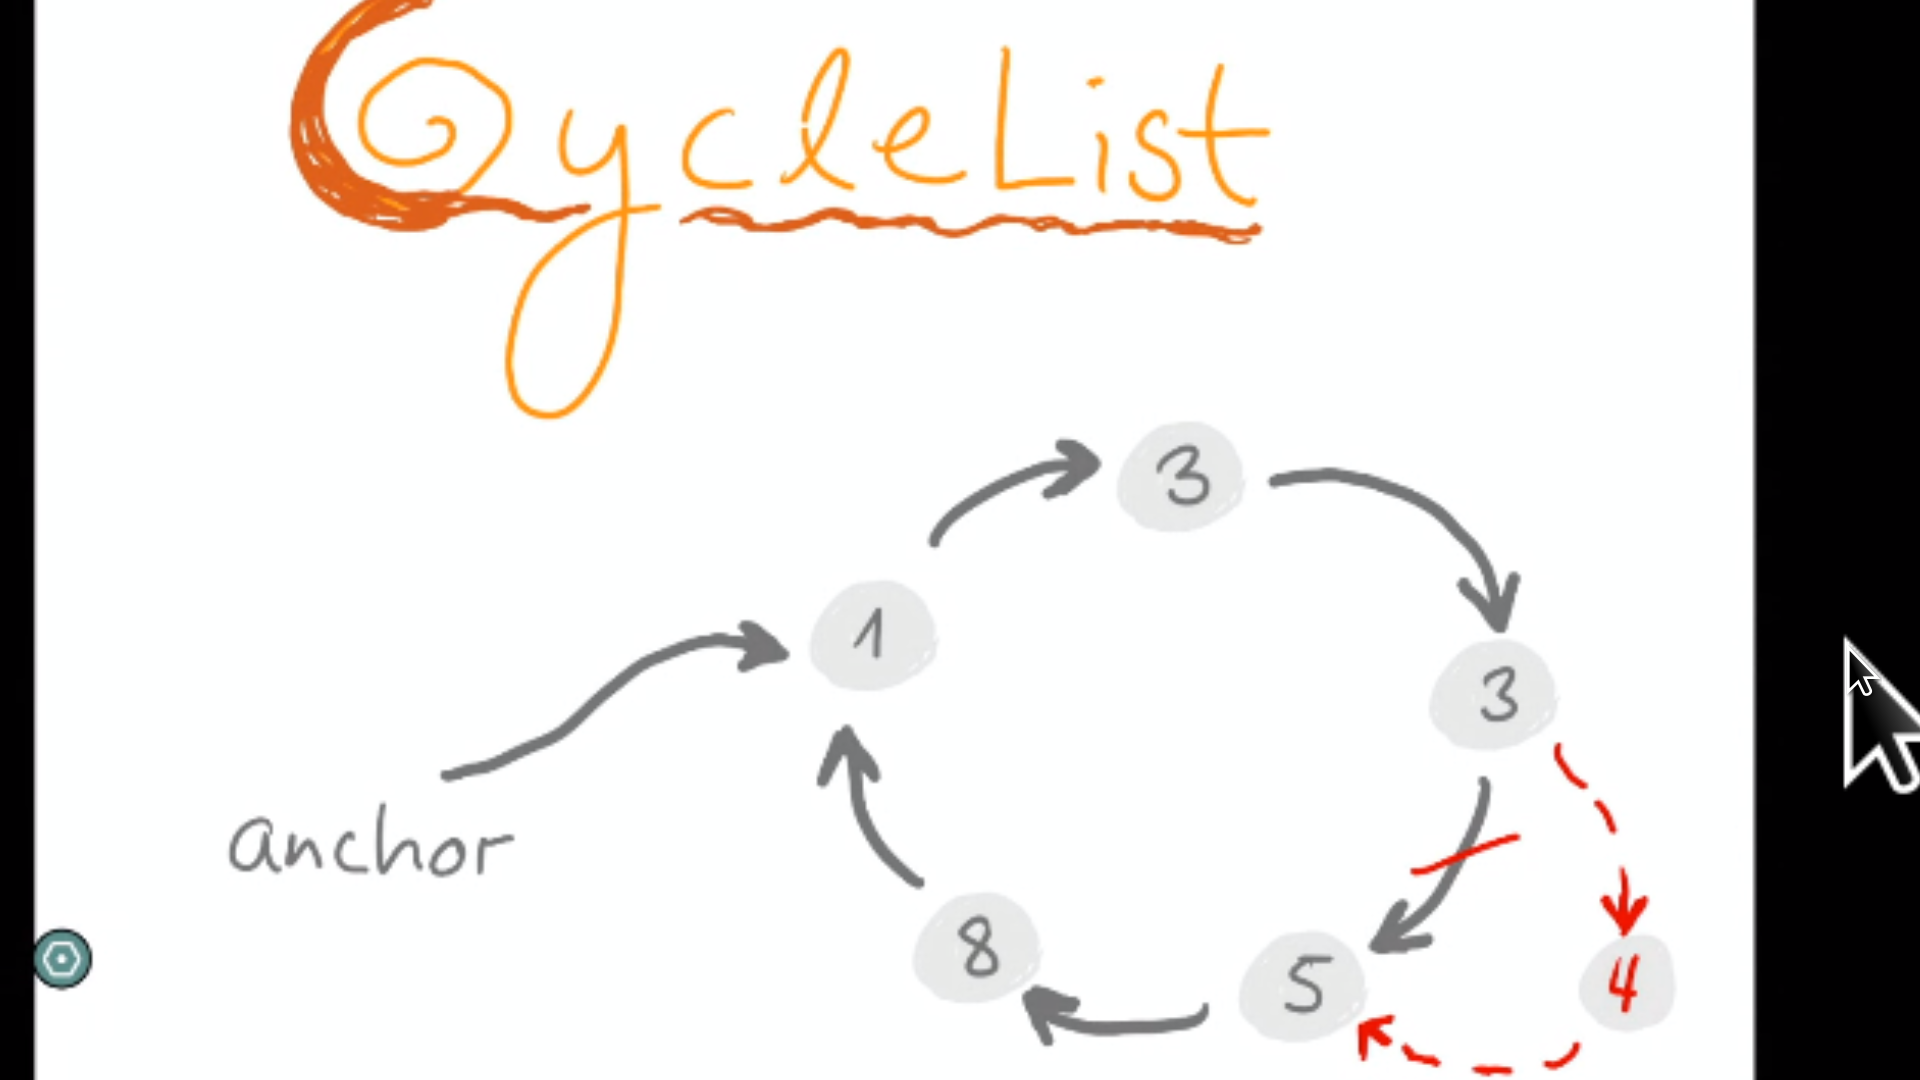
\includegraphics[width=\linewidth]{CList} \\
 	Beispiel für eine Liste ohne Verwaltungsknoten. \\
 	Anker zeigt auf ersten Knoten. \\
 	\subsection*{07.06.2021}
 	Suchbaum \\
 	linker Subbaum immer kleiner als der rechte bezogen auf Schlüssel \\
 	implementieren Sets und Maps \\
 	Set Knoten nur Schlüssel \\
 	Map Knoten enthält neben Schlüssel noch Nutzdaten \\
 	\subsection*{14.06.2021}
 	Hash-Funktionen \\
 	statische Datenstruktur \\
 	im AVG Case hochperformant\\
 	HF Beispiel $h(k) = k mod N$ \\
 	Hashfunktion bildet Objekte auf Position in Hashtabelle ab. \\
 	Hashfunktion braucht konstanten Aufwand. \\
 	mod N Standardoperation \\
 	Jeden Buchstaben im String hashen \\
 	Häufige Basis 31 \\
 	Bei Langen Strings Überlauf für den Datentyp int \\
 	\subsection*{15.06.2021}
 	Lineare Sondierung Kollisionen vermeiden \\
 	LS Funktion g(m) = (h(k) + m) mod N \\
 	g ist nicht optimal \\
 	Lösung c  $\cdot$ m Schritte \\
 	\subsection*{25.06.2021}
 	2 3 4 Bäume  \\
 	Mehrere Werte pro Knoten erlaubt verallgemeinerter Suchbaum \\
 	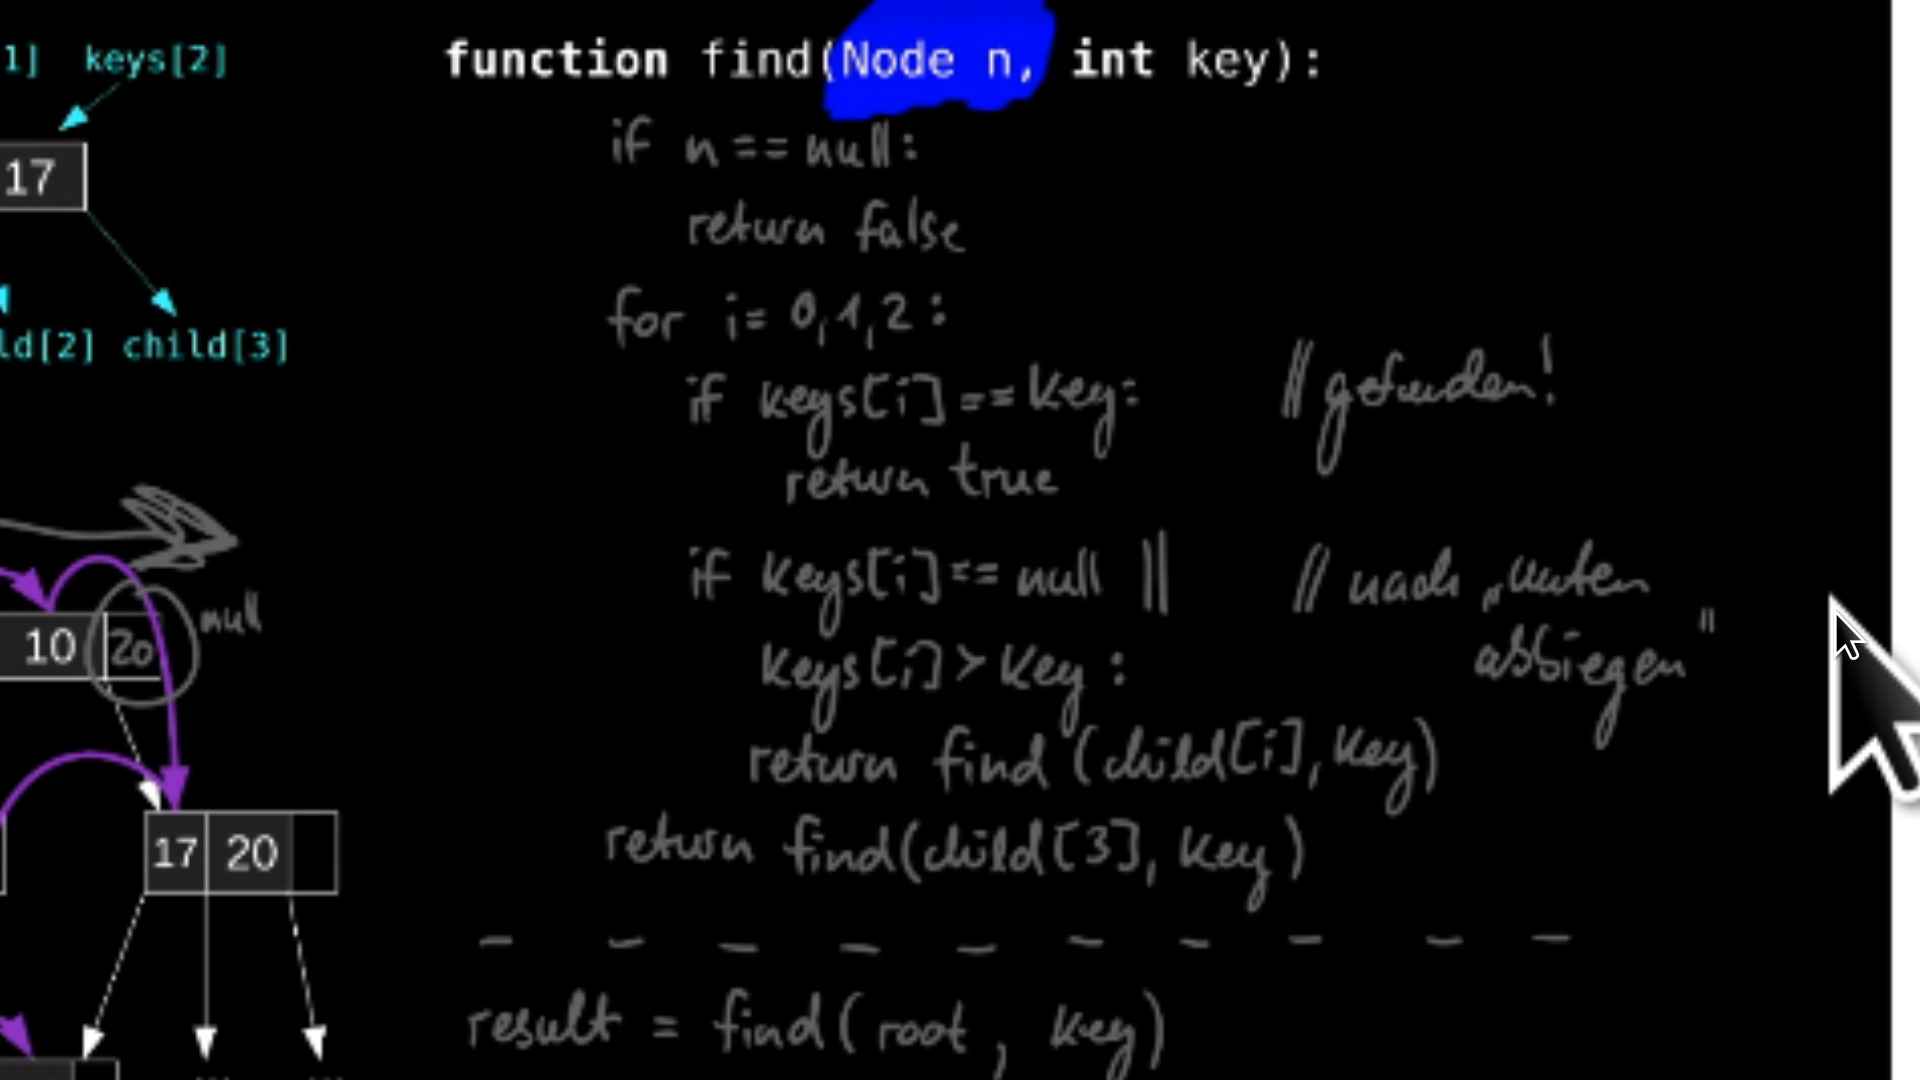
\includegraphics[width=\linewidth]{find} \\
 	2 3 4 Bäume entarten nicht \\
 	Aufwand O(log n) \\
 	Red Black Tree \\
 	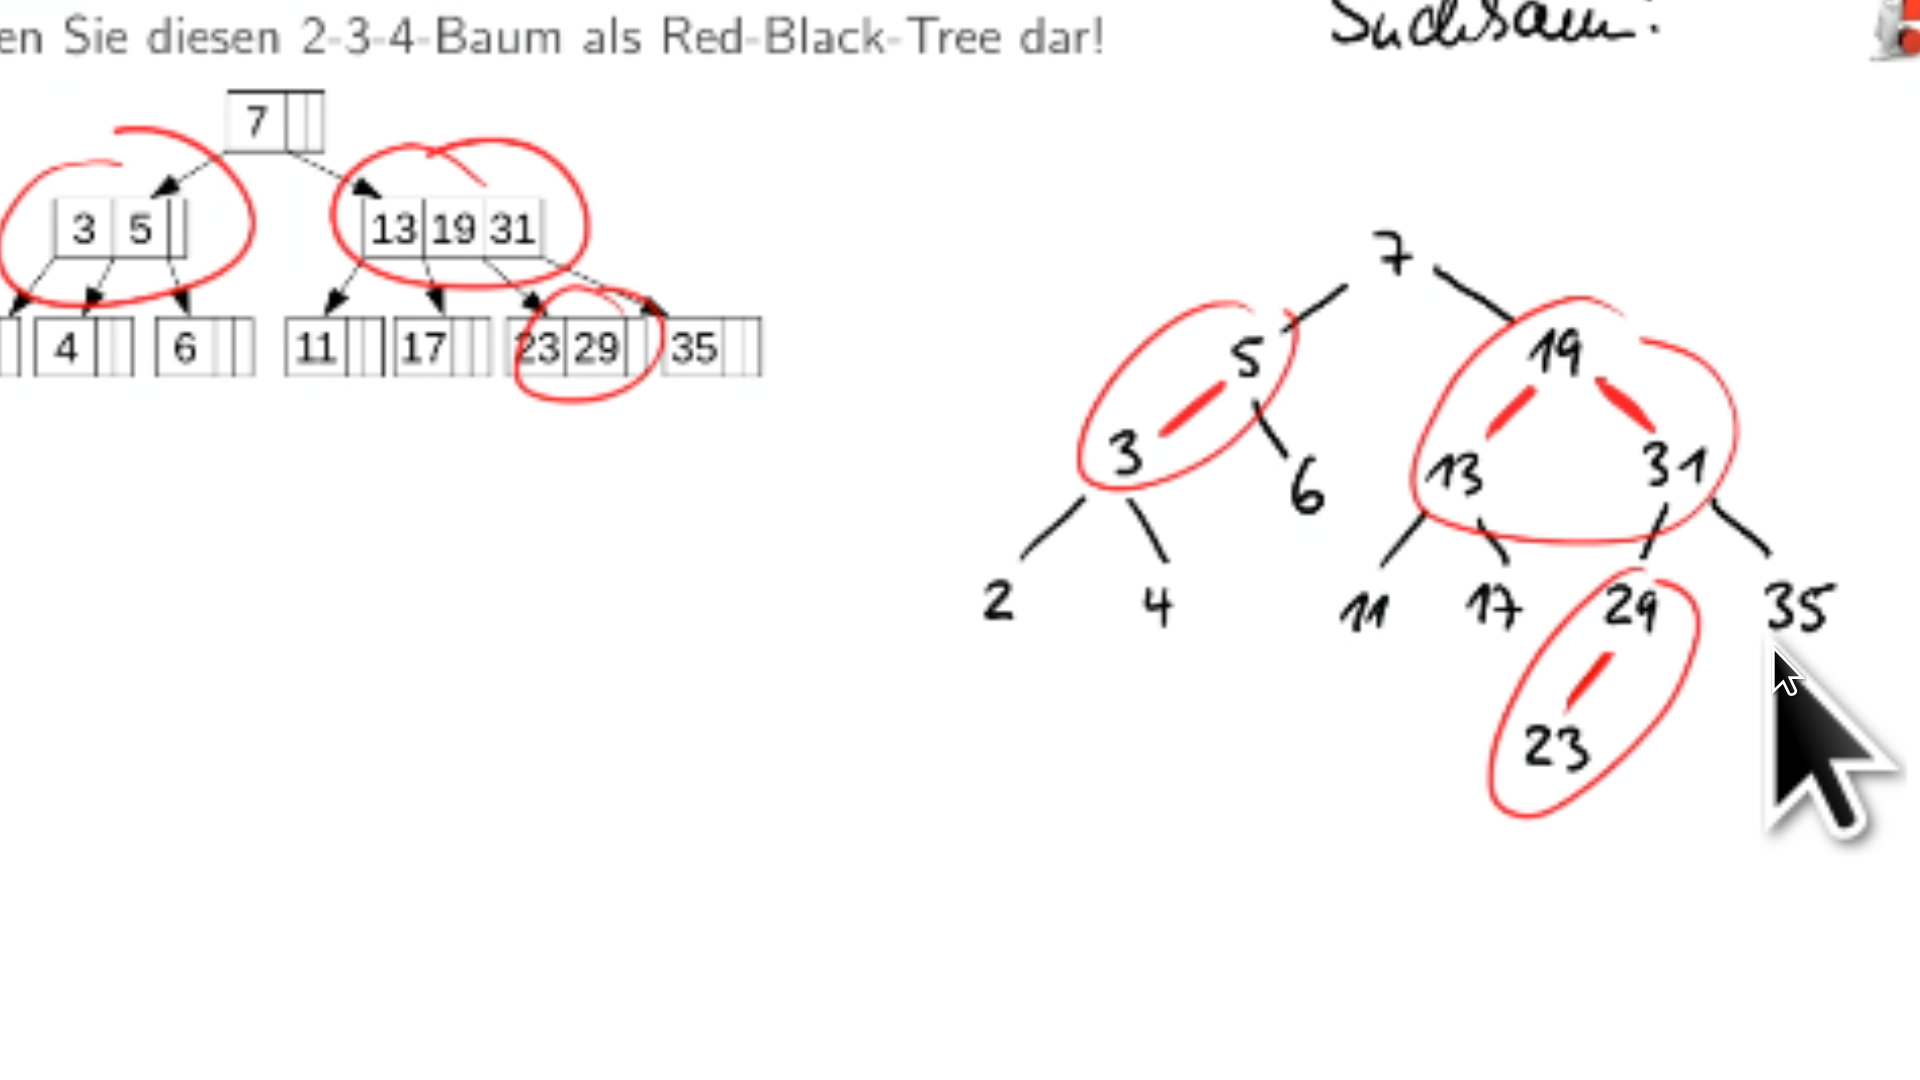
\includegraphics[width=\linewidth]{rbt} \\
	Doppelrotation \\
	Bei Rotation bleibt Suchbaumeigenschaft erhalten. \\
	Teilstruktur verliert an Höhe \\
	\subsection*{02.07.2021}
	RedBlackTrees haben nie zwei aufeinander folgende rote Kanten. \\
	RBT ist O(log n) \\
	Kapitel 10 B-Bäume \\
	2 3 4 Baum hat 1 bis 3 Elemente Pro Knoten \\
	im B Baum wird das bis zur Obergrenze M verallgemeinert. \\
	Schlüssel sind aufsteigend sortiert. \\
	m für tatsächliche Schlüsselzahl \\
	Knoten ist minimal halbvoll und darf maximal ganz voll sein. \\
	In der Wurzel befindet sich nur 1 Wert. \\
	Branch-Faktor = M + 1 \\
	%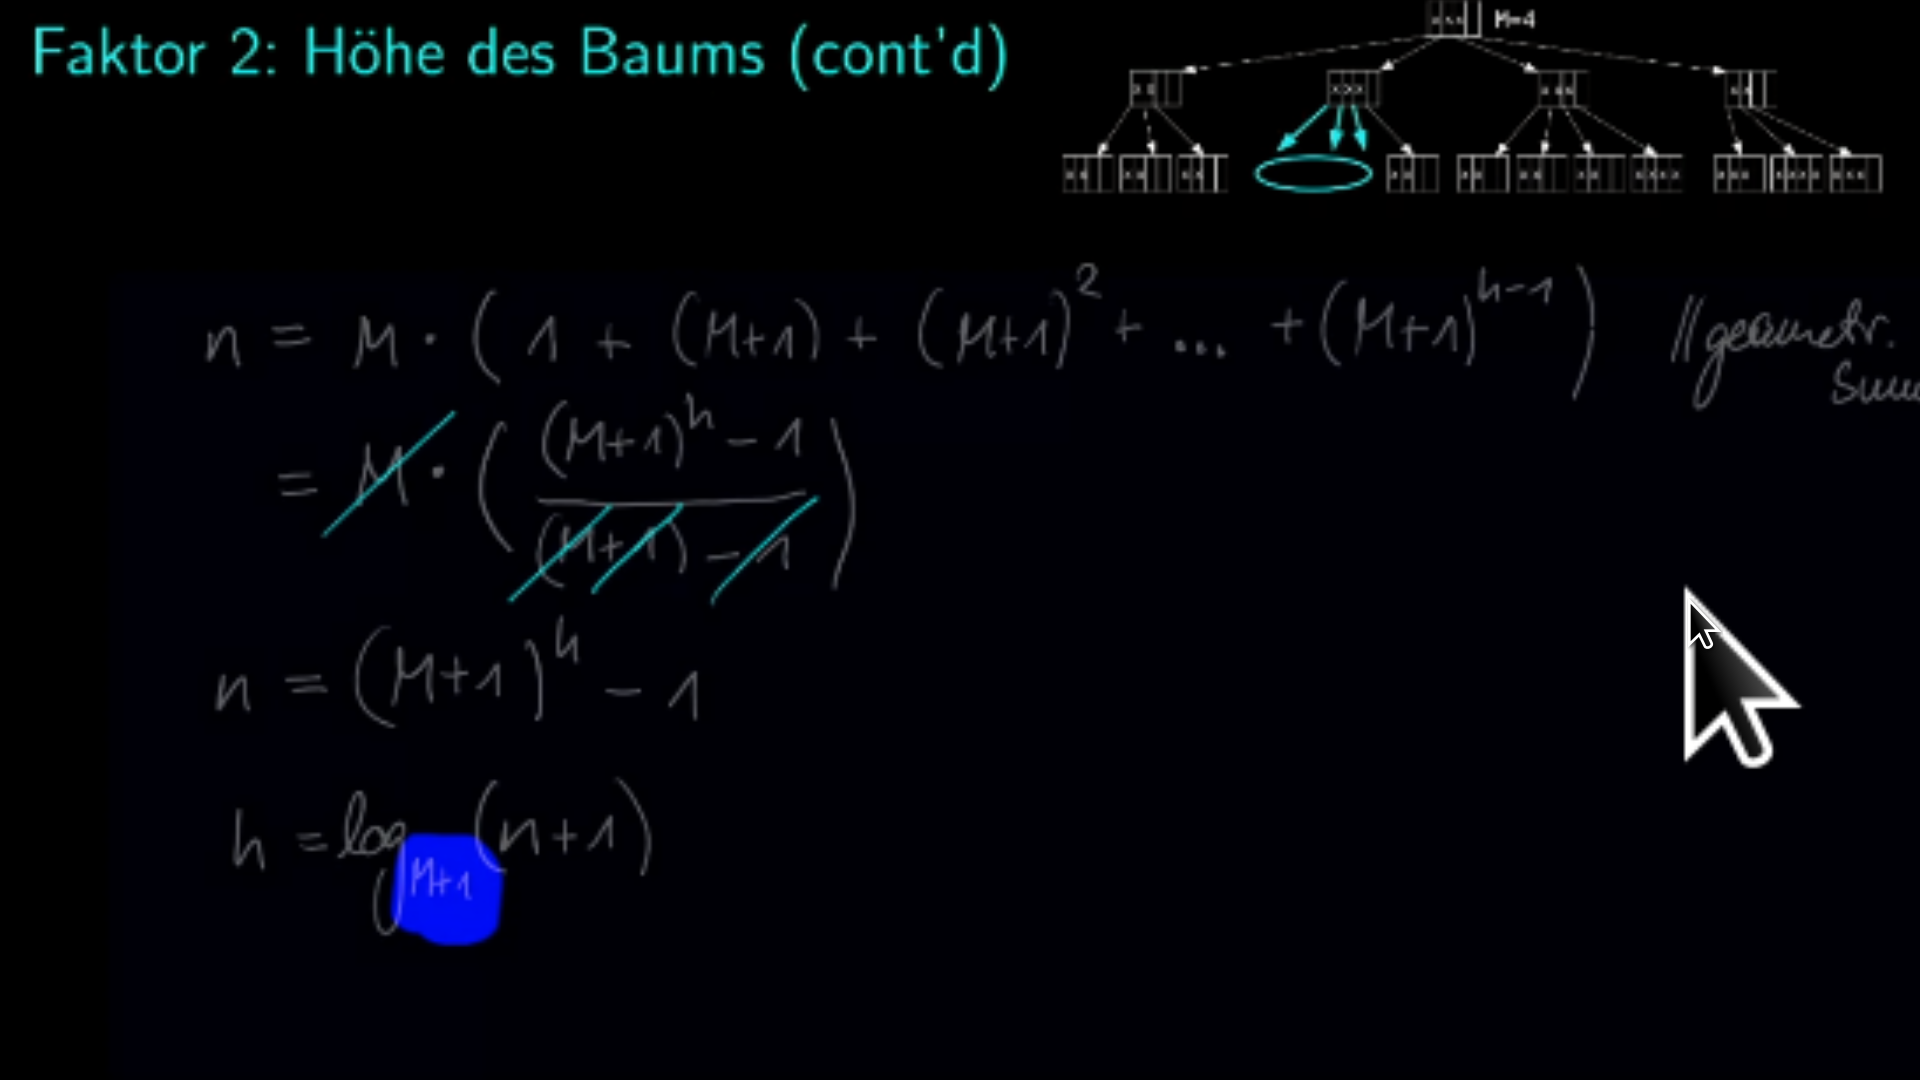
\includegraphics[width=\linewidth{bshot}
	%\includegraphics[width=\linewidth]{bbaumh}
 	BBäume sind seitenoptimiert
	
\end{document}